
\section{Theorie}
\label{sec:Theorie}

Ziel des Versuches ist eine zerstörungsfreie Untersuchung ortsabhängiger Vorgänge. Dazu gehören sowohl die Bestimmung der 
Spin-Gitter-Relaxationszeit $T_1$ und der Spin-Spin-Relaxationszeit $T_2$ als auch die Messung des Diffusionskoeffizienten $D$
von Flüssigkeiten mithilfe der magnetischen Resonanz an Protonen.

\subsection{Spin-Echo-Verfahren}

In diesem Verfahren ist eine Probe von einem möglichst homogenem externen Magnetfeld $\vec{B_0}$ umgeben, wodurch sich die 
magnetischen Momente und die daran gekoppelten Spins der Kerne parallel zu $\vec{B_0}$ ausrichten. 
Diese Orientierungen ergeben eine makroskopische Magnetisierung
$\vec{M}$ der Probe. Durch Anlegen eines magnetischen Wechselfeldes werden die Spins aus ihrer Ausgangslage
parrallel zu $\vec{B_O}$ ausgelenkt und relaxieren nach den charakteristischen Zeiten $T_1$ und $T_2$ wieder zurück.
Dabei führen ihre magnetischen Momente eine sogenannte Lamorpräzession mit der Lamorfrequenz 
$\omega_\text{L} \approx \SI{21.7}{\mega\hertz}$ um die $B_0$-Achse durch und die zeitliche
Änderung von $\vec{M}$ kann durch die Blochschen Gleichungen
\begin{equation}
    \frac{\text{d}M_x}{\text{d}t} = \gamma B_0 M_y - \frac{M_x}{T_2} \qquad 
    \frac{\text{d}M_y}{\text{d}t} = - \gamma B_0 M_x - \frac{M_y}{T_2} \qquad
    \frac{\text{d}M_z}{\text{d}t} = \frac{M_0 - M_z}{T_1}
\end{equation}
mit gyromagnetischem Verhältnis $\gamma$ beschrieben werden.

Dabei umfassen die ersten Terme die Präzession in der x,y-Ebene und die letzteren Terme die Relaxationen.
$T_1$ beschreibt die zu $\vec{B_0}$ longitudinale Spin-Gitter-Relaxation bei der die Kernspinenergie in Gitterschwingungen übergeht
und $T_2$ die transversale Spin-Spin-Relaxation durch Wechselwirkung mit dem nächst benachbarten Spin.

Auf die magnetischen Momente wirkt schließlich ein Drehmoment
\begin{equation}
    \vec{D} = \vec{M} \times B_0 \vec{\text{e}_z} \; .
\end{equation} 

Die beiden Relaxationen werden nach der Spin-Echo-Methode durch eine Auslenkung von $\SI{90}{\degree}$
und eine dadurch resultierende Spinausrichtung senkrecht zu $\vec{B_0}$ hervorgerufen.
Für die transversale Magnetisierung ergibt sich also der mit der Zeit exponentiell abnehmende Verlauf
\begin{equation}
    M_\text{x,y} \left(\tau\right) = M_0 \exp{\left(-\frac{2\tau}{T_2}\right)} \; .
    \label{eqn:MGM}
\end{equation}
Damit erstarkt die longitudinale Magnetisierung mit dem Verlauf 
\begin{equation}
    \begin{equation}
        M_\text{z}\left(\tau\right) = M_0 \left(1-2\exp{\left(-\frac{\tau}{T_1}\right)}\right) \; .
        \label{eqn:SGR}
    \end{equation}
\end{equation}

Bei Anlegung eines auf den $\SI{90}{\degree}$ folgenden $\SI{180}{\degree}$-Pulses relaxieren die Spins erst nach einer Zeit $T$
und erzeugen dadurch ein Spin-Echo-Signal. Dieses Verfahren ist schematisch in \ref{fig:spinecho} dargestellt.

\begin{figure}
    \centering
    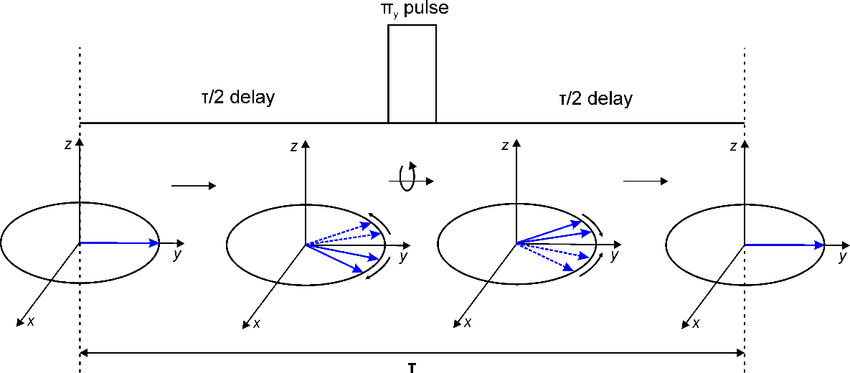
\includegraphics[scale=0.4]{content/spinecho.png}
    \caption{Typische Spin-Echo-Sequenz \cite{spinecho}.}
    \label{fig:mgm}
  \end{figure}

  Die Methode der Carr-Purcell-Pulzsequenz erlaubt eine Bestimmung von $T_2$ indem statt einem mehrere
  $\SI{180}{\degree}$-Pulse hinter einander geschaltet werden. Die Spin-Echos werden nach dieser
  Methode mit der Zeit kleiner, da sich immer mehr Spins durch $\vec{B_0}$ ausrichten.
  Es ergiben sich für verschiedene Atome unterschiedliche charakteristische Relaxationszeiten, 
  die gemessen werden und duch die z.B. Verbindungen genauer untersucht werden können.
  Die Meiboom-Gill-Methode basiert auf einer ähnlichen um \SI{90}{\degree} phasenverschobenen Pulsfolge, 
  die ein alternierendes Vorzeichen der Amplitude besitzt. Durch diese Verschiebung heben sich die 
  Ungenauigkeiten des Drehwinkels auf.

\subsection{Feldgradienten-NMR}

Um z.B. die Diffusion von Molekülen durch Brownsche Eigenbewegung als ortsänderlichen Prozess zu untersuchen, 
wird ein magnetisches Wechselfeld mit Resonanzfrequenz an die Probe angelegt. Dadurch 
können bei bekanntem Feldgradienten eine ortsabhängie Resonanzfrequenz gemessen werden, die 
Aufschluss über jene Ortsabhängigkeit gibt.

In Folge einer Diffusion können Protonen in Probenbereiche vordringen, in denen ihre Lamorfrequenz nicht mehr
mit dem änderlichen $\vec{B}$ resonieren. Deshalb nimmt die Echoampliude zeitlich exponentiell mit
\begin{equation}
    A(2\tau) = \text{exp}\left(\sfrac{1}{3}D \gamma^2 G^2 \tau^2 (2\tau)^2 \right)
\end{equation}
ab. $G$ beschreibt dabei den Feldgradienten und $D$ den Diffusionskoeffizienten. Als Zeitkonstante
ergibt sich die Diffusionszeit 
\begin{equation}
    T_D = \frac{3}{D \gamma^2 G^2 \tau^2} \; .
\end{equation}

Dadurch wird der zeitliche Verlauf der transversalen Magnetisierung zu 
\begin{equation}
    M_\text{x,y} \left(2\tau\right) = M_0 \exp{\left(-\frac{2\tau}{T_2}\right)} \exp{\left(-\frac{2}{3}D\gamma^2G^2\tau^3\right)} 
    \label{eqn:DK}
\end{equation}
erweitert. Die Diffusionskonstante ergibt sich mit der Viskosität $\eta$ und dem Molekülradius $r$ zu
\begin{equation}
    D = \frac{k_\text{B}T}{6\pi \eta r} \; .
\end{equation}
